\subsubsection{Move Search and Position Evaluation}

A challenge for both humans and computers is to find the best possible move. In fact, chess is considered unsolved, i.e. it is not known if there is an optimal strategy that always leads to victory, for either sides. The objective of a good chess engine is therefore to find the best move based on its computational capabilities. One factor to consider is the depth of analysis. Thus, each move must be considered not only in terms of the current state of the board, but also what effect it will have on subsequent best moves and positions. In order to find the best move, two tasks must be achieved, one is to find the legal, possible moves in the current and the following positions, and the other is the evaluation of these positions.

To implement these two tasks, many systems such as \Gls{DeepBlue} and earlier versions of \Gls{Stockfish} use human-defined evaluation functions and game tree search algorithms. The evaluation function receives the board as input and evaluates how good the obtained position is. Game tree search algorithms, such as MinMax, are then used to search for all possible moves (Usually, up to a certain depth, e.g. 15 moves). Each move leads to a new position. Since there is no information about these new positions yet, they need to be evaluated by the evaluation function. In the end, the path that has received the highest value from the evaluation function is chosen. Improvements such as alpha-beta pruning remove paths that are known not to yield high values of the evaluation. The problem with this method is that the evaluation functions have to be written by hand with the help of chess experts and constantly refined to achieve an optimal result.

To overcome this problem, and to get the best results from the engine for the commentator, machine learning is used. \cite{alphazero-2018} presented an algorithm that uses Monte Carlo tree search (MCTS) and a neural network. The neural network is used to evaluate an input position. It outputs two pieces of information: A vector with the move probabilities of all next legal moves and, a value, which tells what the player's chances of winning are for the given position. MTCS is used to search deeper, i.e., to search many possible move paths and then select the path with the best neural network evaluation.

\begin{figure}[h]
\centering
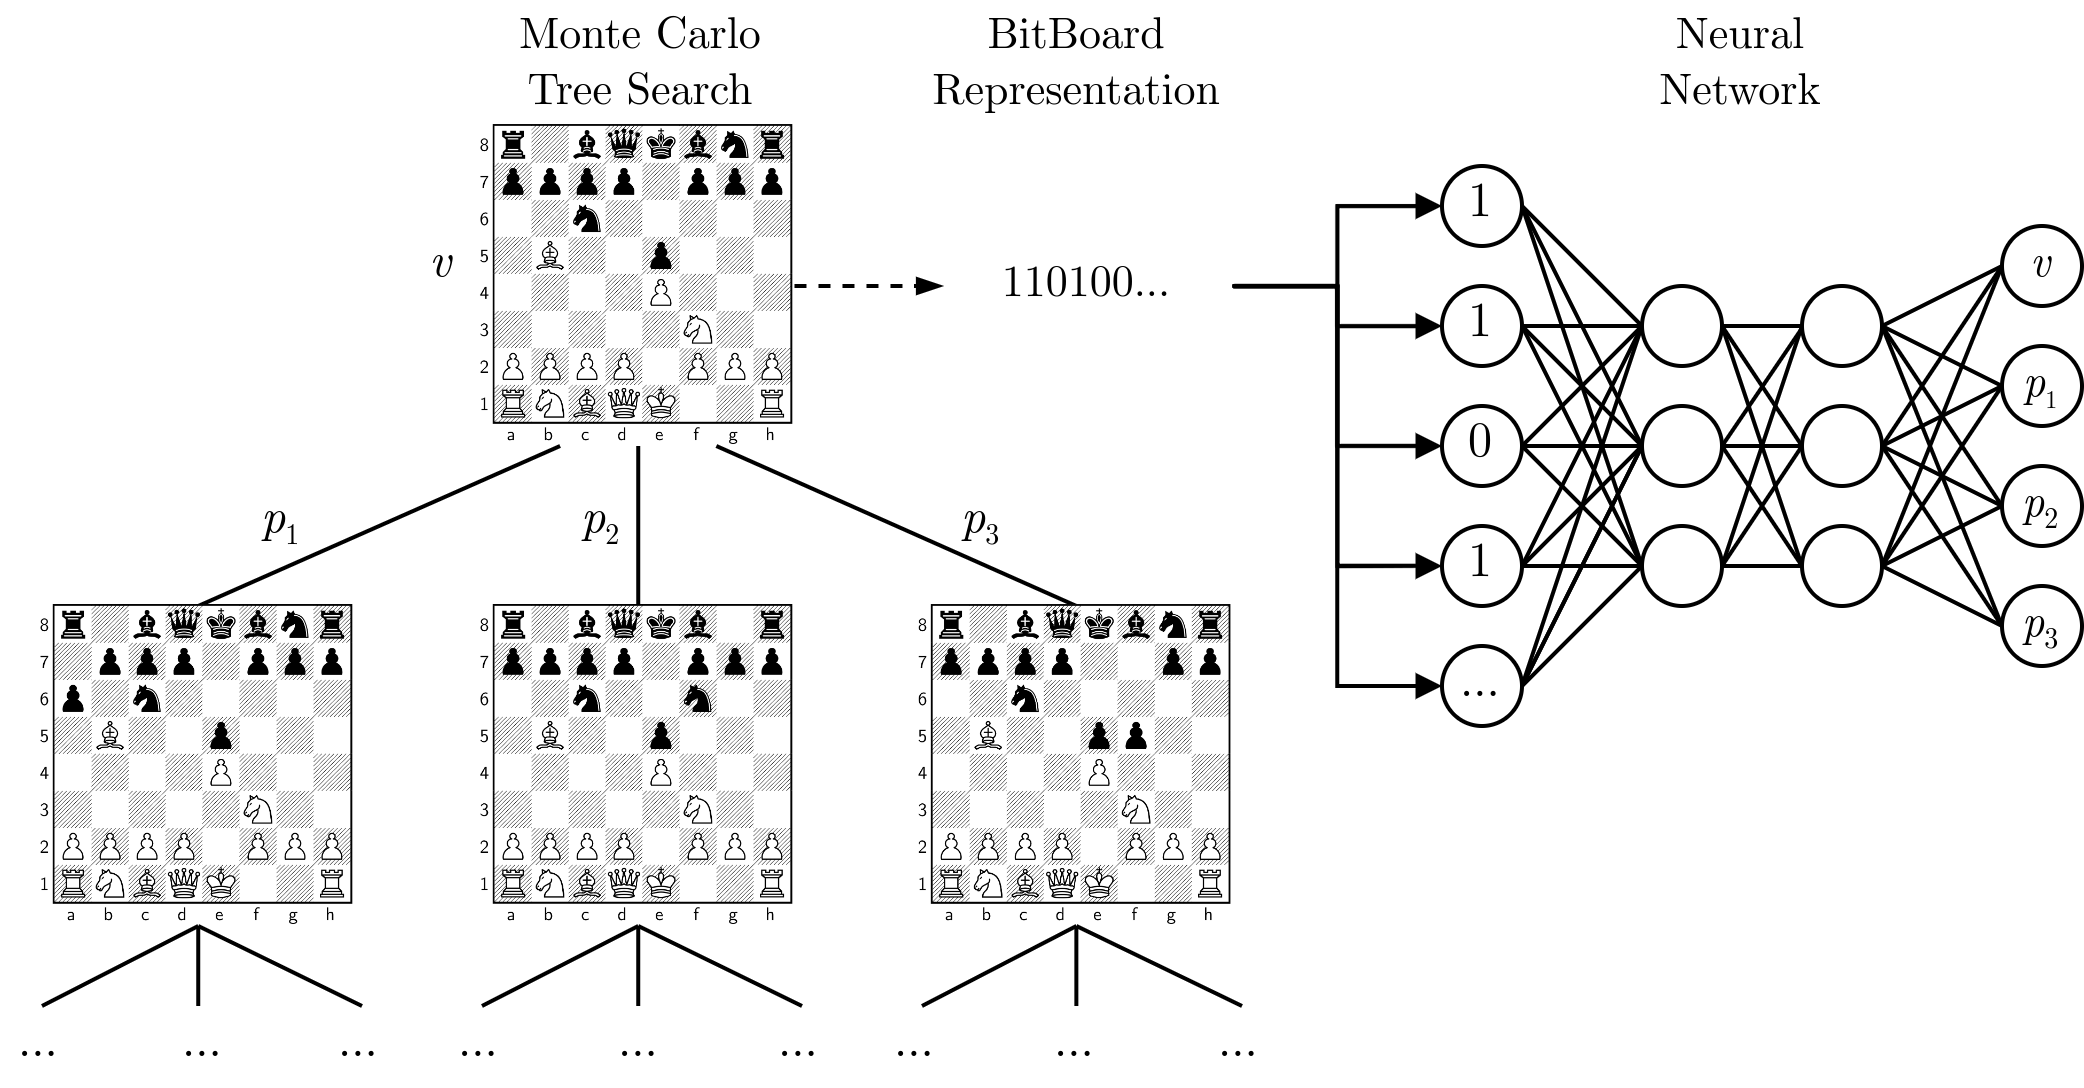
\includegraphics[width=0.95\textwidth]{graphics/alphazero/alphazero.png}
\caption{Simplified example of move search and position evaluation using MCTS and a neural network. ($p_{n}$ move probabilities, $v$ winning chance value)}
\end{figure}

In order for the neural network to deliver the best possible results, it must be trained with data. Instead of relying on existing data sets, \cite{alphazero-2018} used the approach of generating their own data sets through self-play. Initially a program exists that only knows the rules of the game, uses an untrained neural network for evaluation and the MCTS algorithm for move selection. The program executes the following four steps to train the neural network: (1) The program plays against itself by searching for several moves in advance through the MTCS, letting the neural network evaluate these moves for move probability and position strength, and finally choosing the path with the best evaluation. Every game is recorded move by move. At the end of each match, the final position of the sides are assigned lost (-1), drawn (0) or won (+1) to create a dataset.\footnote{See Silver et. al p. 2} (2) The neural network is cloned and the parameters are adjusted "to minimize the error between the predicted result [...] and the game result [...]" and train the network with the generated data set. (3) Let the new program play against the previous one. (4) The winning program is selected and the process is repeated from step 1. As \cite{alphazero-2018}  showed, this method was able to outperform Stockfish, the strongest engine at this time, after only 4 hours.

\begin{figure}[h]
\centering
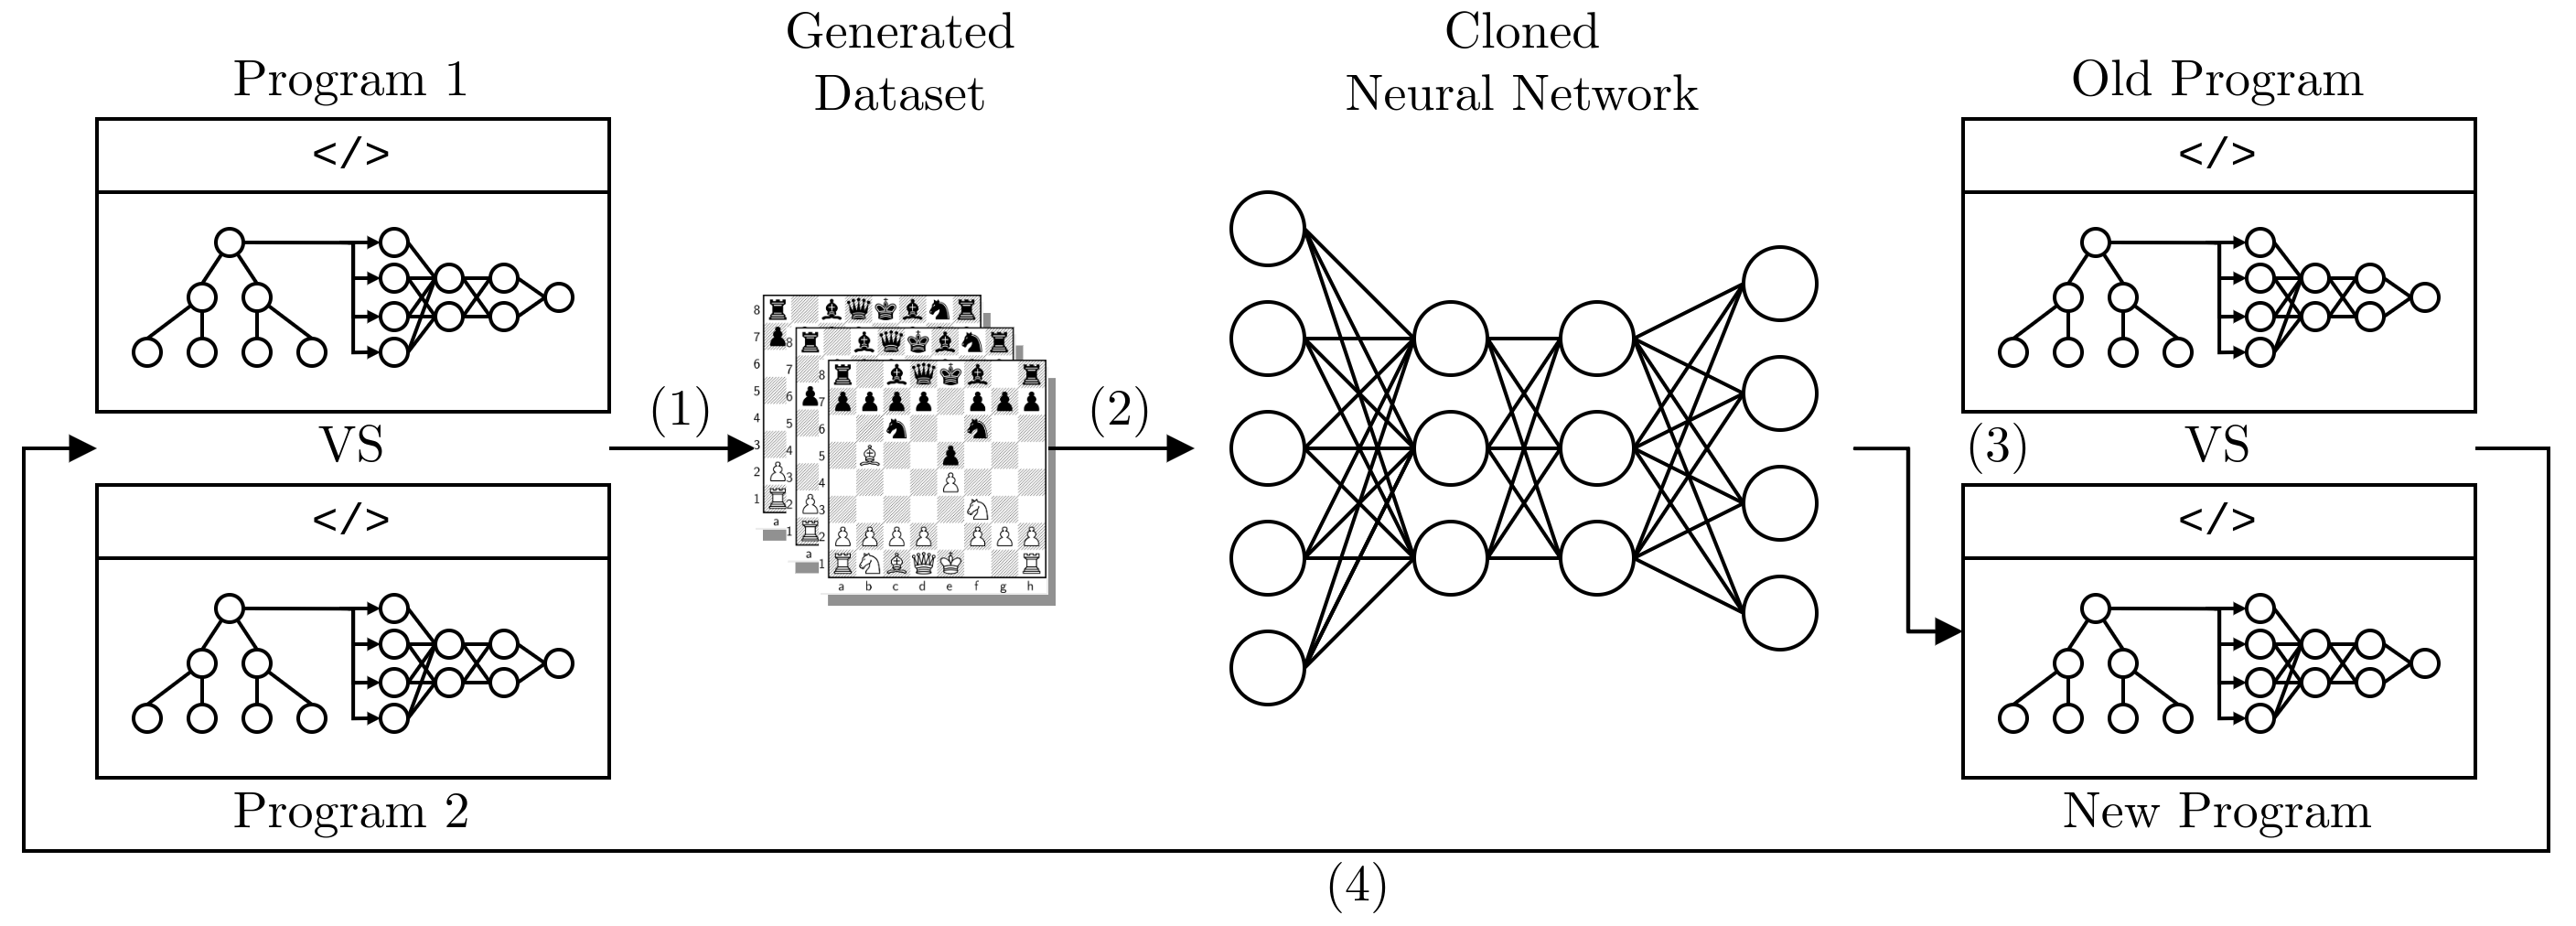
\includegraphics[width=0.95\textwidth]{graphics/alphazero/selfplay.png}
\caption{Steps of traning the neural network through self-play}
\end{figure}